\documentclass[a4paper,12pt]{article}

% Pacotes essenciais
\usepackage[utf8]{inputenc}
\usepackage[T1]{fontenc}
\usepackage[brazil]{babel}
\usepackage{amsmath, amssymb}
\usepackage{graphicx}
\usepackage{geometry}
\usepackage{hyperref}
\usepackage{float}
\usepackage{indentfirst}

% para por código com corzinha ui ui 
\usepackage{minted}
\usepackage{xcolor}

\definecolor{bg}{rgb}{0.1,0.1,0.1}
\usemintedstyle{monokai}

\geometry{a4paper, margin=2.5cm}

\begin{document}

\begin{titlepage}
    \centering

    \vspace*{5cm}
    
    {\LARGE Documentação do Seed++\par}

    \vspace{2cm}

    {\Large Francisco Passos dos Santos Alves\par}

    \vfill

    São Cristóvão, SE \\
    Abril 2026

\end{titlepage}
\clearpage
\pagenumbering{arabic}


\newpage
\tableofcontents
\newpage


\section{Introdução}

O Seed++ (ou Seed Plus Plus) é um dispositivo baseado em sistema embarcado, projetado para o laboratório de Física 
da FnEsc, com o objetivo de controlar o acesso ao ambiente, permitindo a entrada apenas de pessoas autorizadas. 
O projeto foi desenvolvido com foco na aplicação prática de paradigmas de programação, como Programação Orientada a 
Objetos (OO).

O sistema do Seed++ permite a realização de operações de CRUD (Create, Read, Update, Delete) sobre os usuários quando se encontra no modo administrador, que será detalhado na seção de funcionalidades. No modo de leitura, apenas usuários previamente cadastrados podem acessar o laboratório de forma controlada.

A arquitetura do sistema foi projetada de forma modular, separando responsabilidades em camadas como drivers de hardware, lógica 
de aplicação e aspectos transversais, como segurança e auditoria. Essa abordagem contribui para a manutenção, escalabilidade e 
confiabilidade do sistema.


\section{Visão Geral do Sistema}

O Seed++ é um sistema embarcado baseado em Arduino Nano que integra um leitor RFID via protocolo de comunicação 
SPI, um solenoide controlado por relé, um display LCD com adaptador para comunicação por protocolo I2C, LEDs 
indicadores e botões multiplexados. A arquitetura foi projetada em cinco camadas: core (orquestrador central),
drivers (abstração de hardware), logic (lógica de funcionamento), storage (gerenciamento de dados em EEPROM) 
e aspects (preocupações transversais com programação orientada a aspectos).

O sistema opera em dois modos distintos. No modo Leitura, o dispositivo valida cartões RFID contra uma 
lista de autorizados armazenada em EEPROM, acionando o solenoide para liberar acesso. No modo Administrador,
um usuário com acesso privilegiado pode gerenciar cadastros através de botões multiplexados, permitindo criar, 
deletar ou modificar registros de usuários.


\section{Arquitetura}

\subsection{Hardware}

\subsubsection{Estrutura Modular}
O Seed++ foi desenvolvido com uma abordagem modular, consistindo em dois módulos principais interconectados via 
conectores header: o Módulo de Controle e Alimentação e o Módulo de Interação. Esta separação física reflete a 
separação lógica entre componentes críticos de controle e interface do usuário.

\subsubsection{Módulo de Controle e Alimentação}
Este módulo gerencia a alimentação do sistema, operando com tensões de 12V e 5V. Contém o Arduino Nano como 
microcontrolador central, o módulo regulador de tensão step-down (12V para 5V) e o módulo relé para controle 
do solenoide. O módulo de alimentação é responsável pela lógica central e acionamento da tranca.

\subsubsection{Módulo de Interação}
Este módulo concentra toda a interface com o usuário, operando com tensões de 3.3V e 5V. Inclui o display LCD I2C, o 
módulo RFID, LEDs indicadores (vermelho, verde e admin), botões multiplexados no pino analógico A0 e a chave de segurança
para modo administrador. O módulo de interação possui acesso a todos os pinos do Arduino Nano, permitindo máxima flexibilidade
na configuração e expansão futura do sistema.

\subsubsection{Interconexão entre Módulos}
Os dois módulos são interconectados via conectores header, transmitindo sinais digitais e analógicos, bem como
tensões de alimentação (3.3V, 5V e GND) necessárias para operação coordenada do sistema.


\subsubsection{Diagrama Esquemático}

\begin{figure}[ht]
\centering
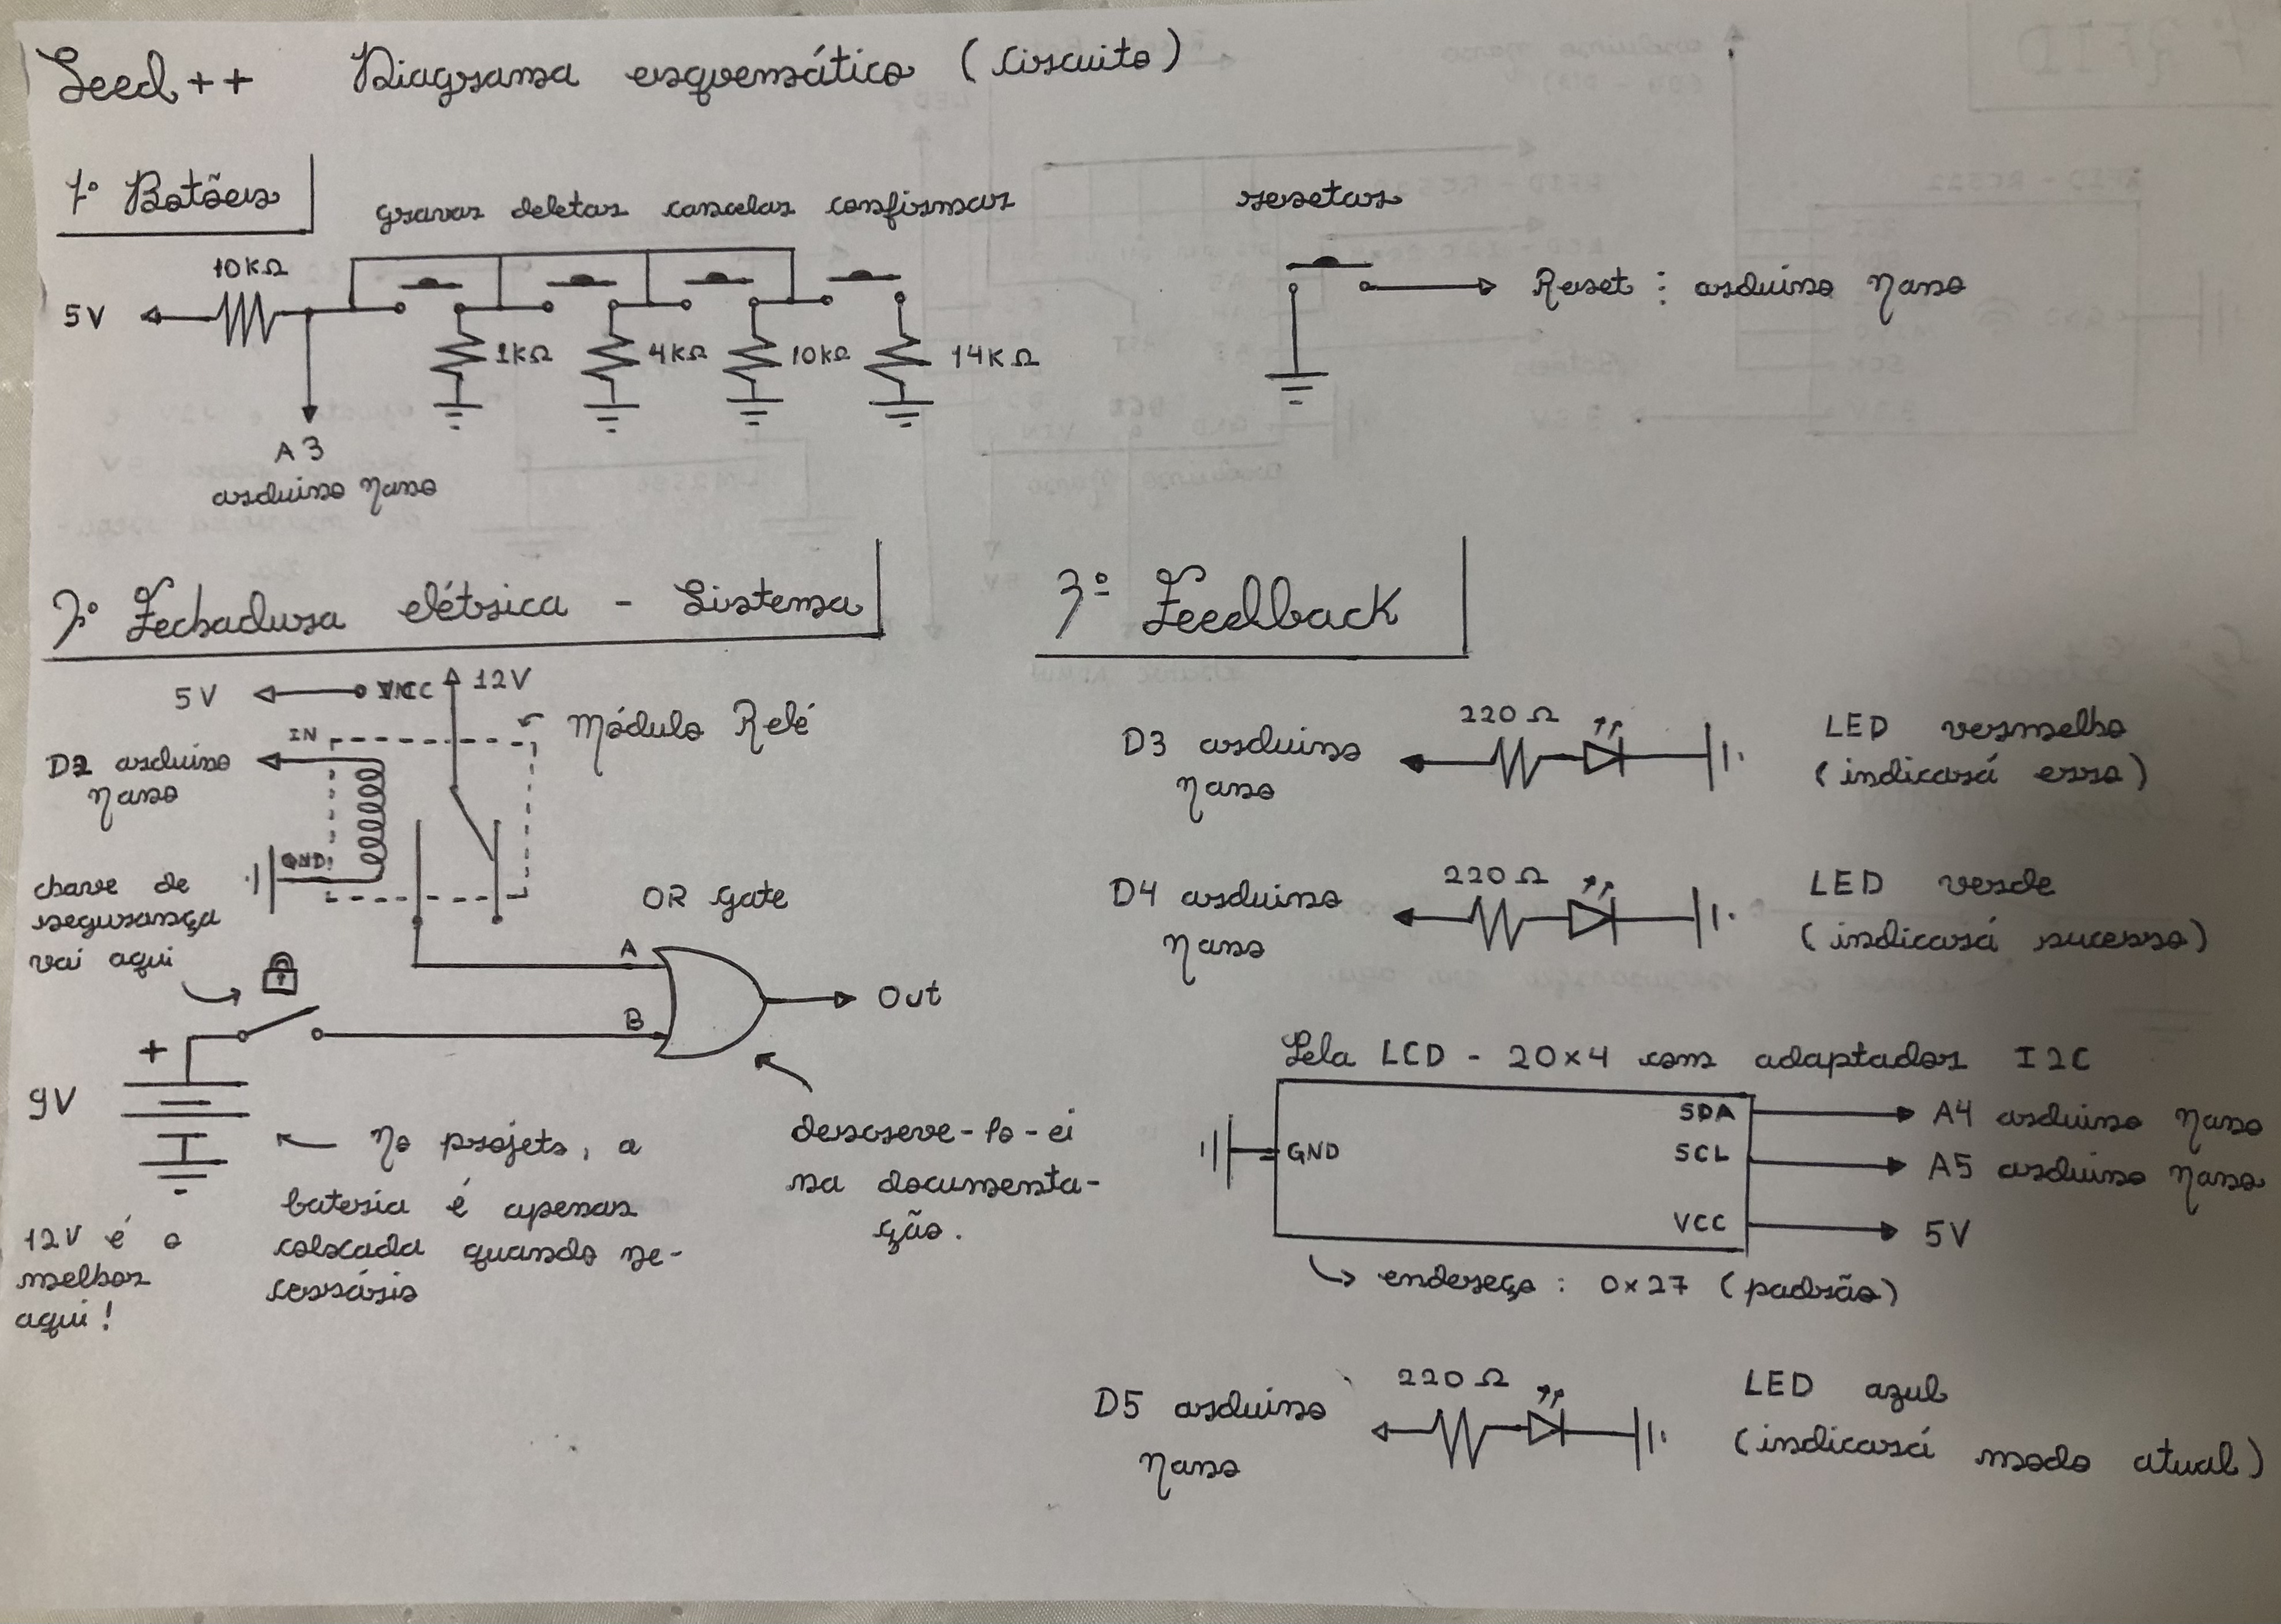
\includegraphics[width=0.8\textwidth]{../assets/esquematico-1.png}
\caption{Diagrama esquemático do Seed++}
\label{fig:schematic1}
\end{figure}

\begin{figure}[ht]
\centering
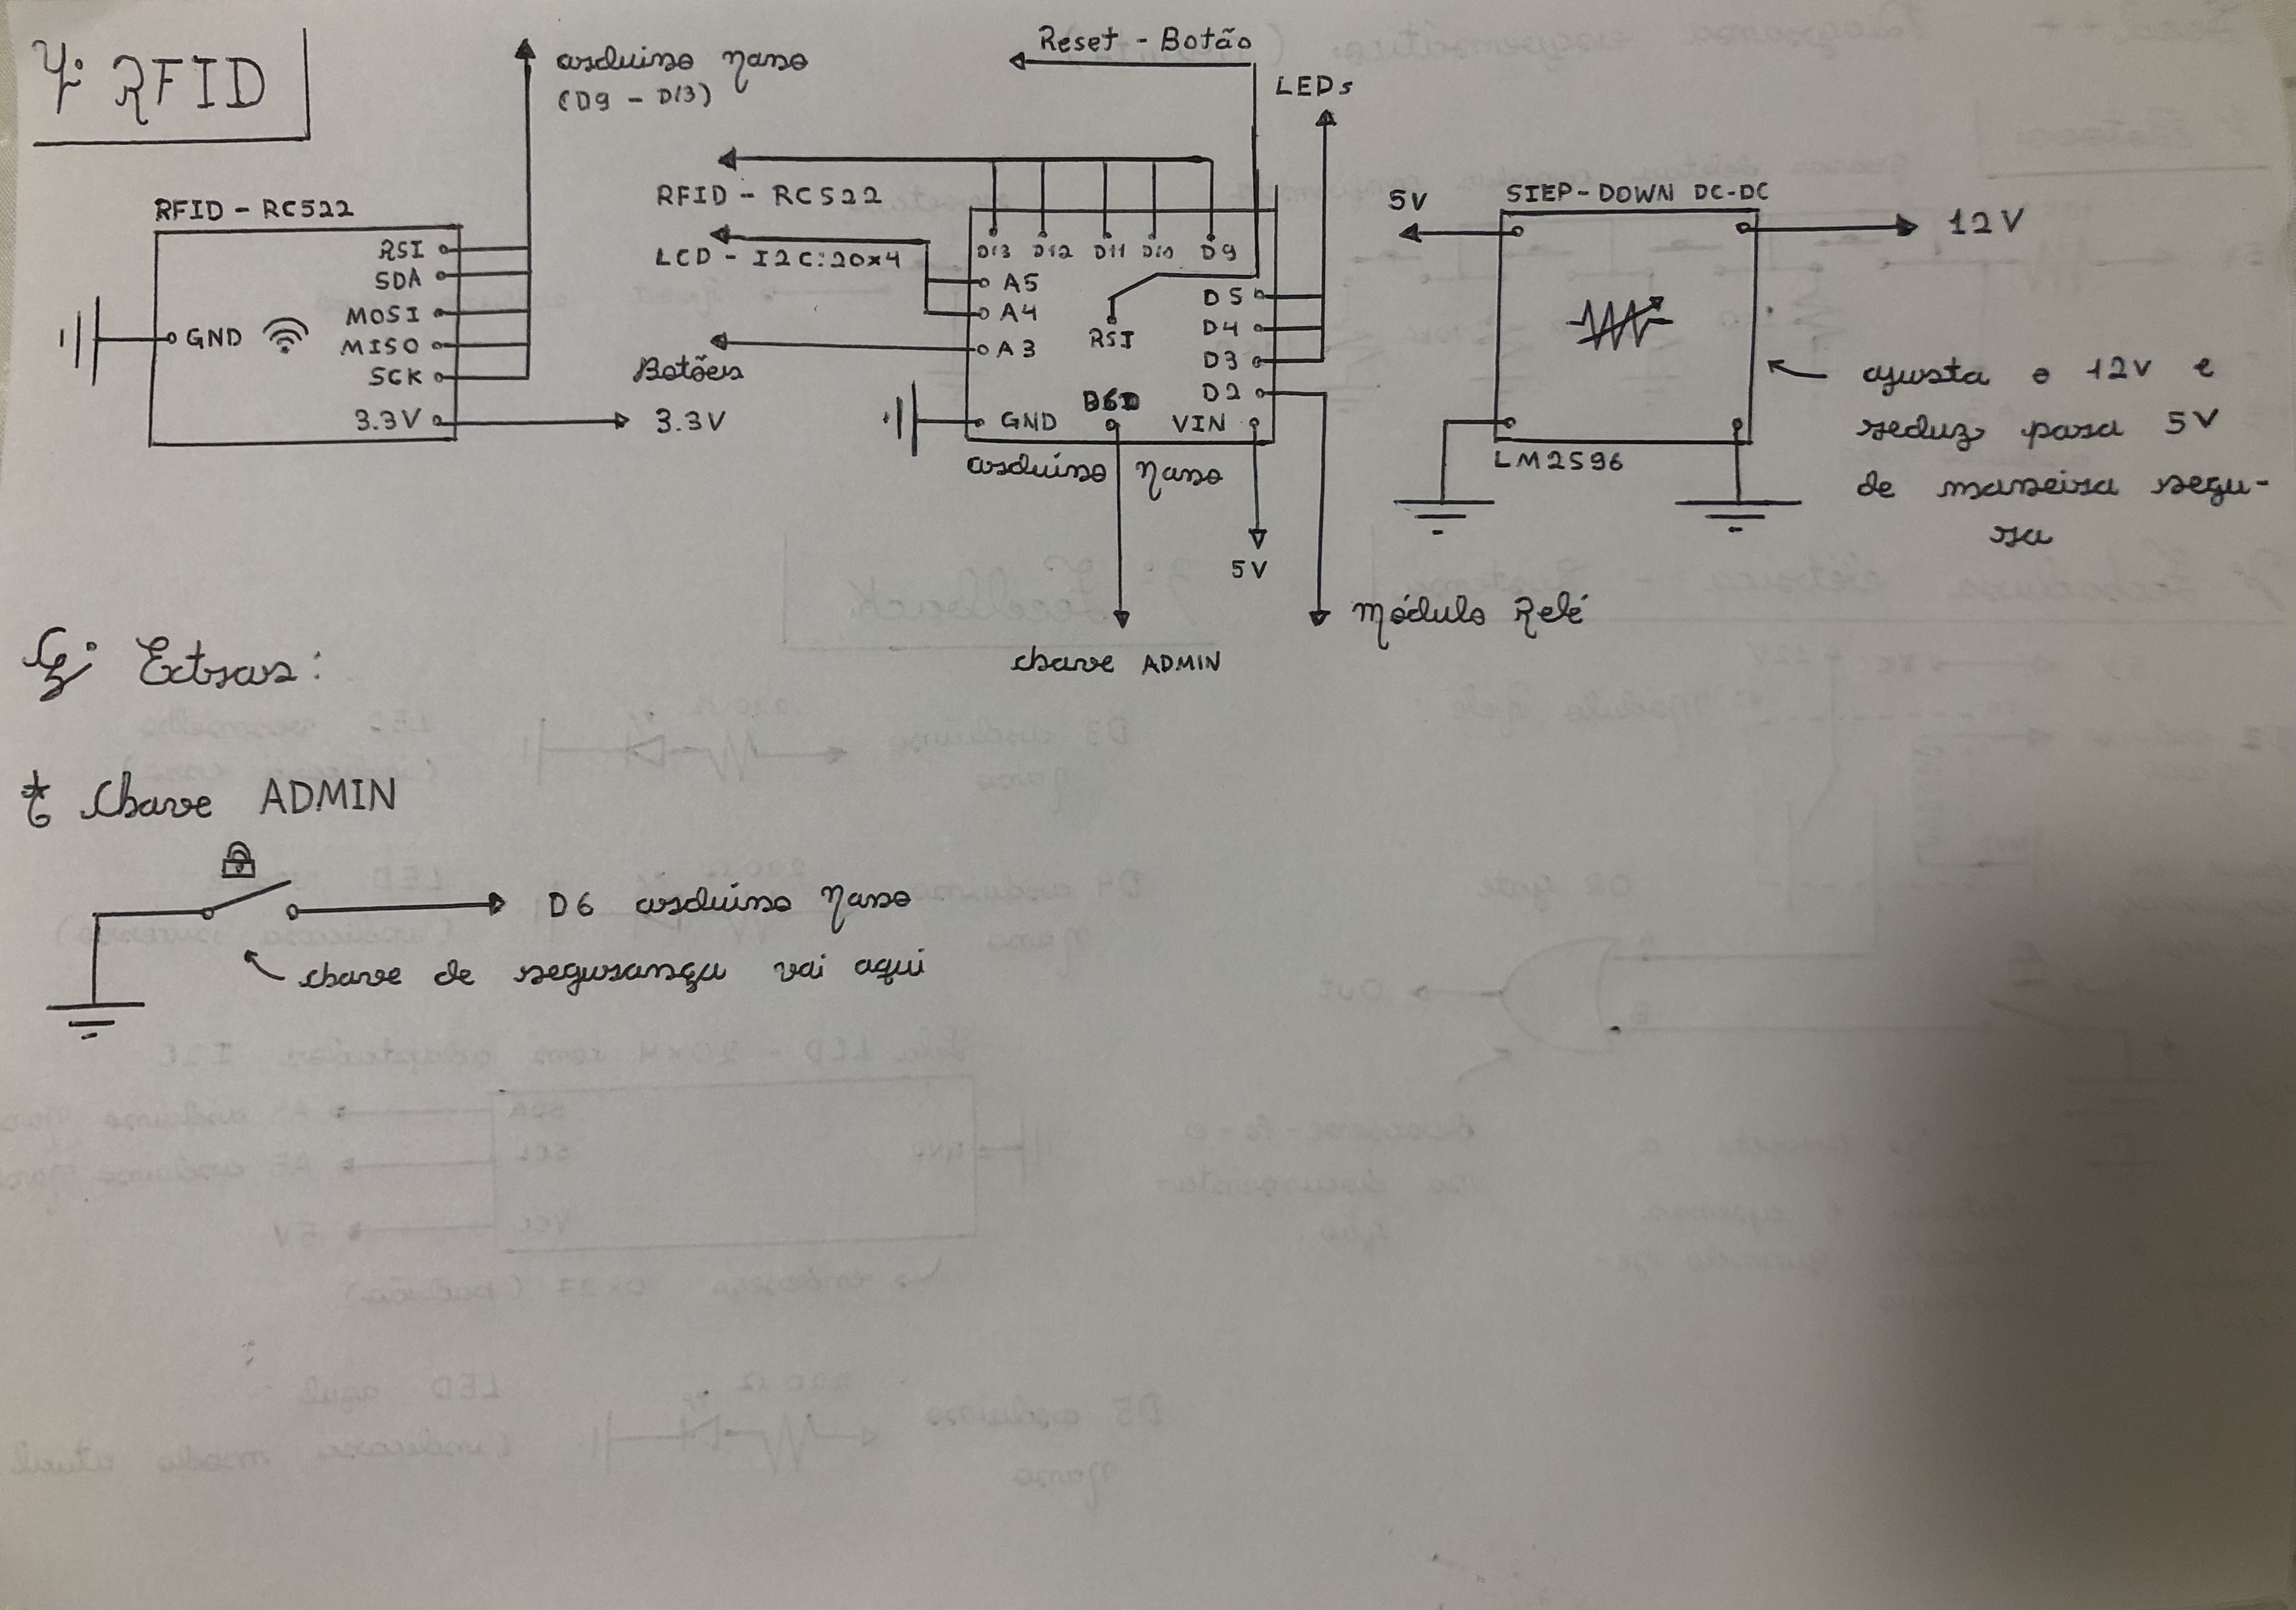
\includegraphics[width=0.8\textwidth]{../assets/esquematico-2.png}
\caption{Diagrama esquemático do Seed++}
\label{fig:schematic2}
\end{figure}

\newpage


\subsection{Software}


\section{Componentes do Sistema}


\section{Modo de Operação}

\subsection{Leitura}

\subsection{Administrador}


\newpage
\section{Informações de Contato}

Para dúvidas, sugestões ou contribuições relacionadas ao projeto Seed++, entre em contato:

\begin{itemize}
    \item GitHub: \url{https://github.com/franksteps/seed-plus-plus}
    \item LinkedIn: \url{https://www.linkedin.com/in/franksteps/}
    \item E-mail pessoal:       franciscopassos.contato@gmail.com
    \item E-mail acadêmico:     francisco.alves@dcomp.ufs.br
    \item E-mail profissional:  contato@franksteps.com.br
\end{itemize}


\end{document}
